\graphicspath{{chapters/exercises_sections/exercises_images/}}
\section{Multidimensional integrals}
  
  \subsection{Computing multidimensional integrals}
  Compute $\int\limits_{y=0}^{y=\pi}\int\limits_{x=y}^{x=\pi}\frac{sinx}{x}dxdy$.
  \begin{align*}
    \int\limits_{y=0}^{y=\pi}\int\limits_{x=y}^{x=\pi}\frac{sinx}{x}dxdy 
      & = \int\limits_{x=0}^{x=\pi}\int\limits_{y=0}^{y=x}\frac{sinx}{x}dydx 
      & \text{change order of integration}\\
      & = \int\limits_{x=0}^{x=\pi} \left[y\frac{sinx}{x}\right]_{y=0}^{y=x}dx
      & \text{integrate over y} \\
      & = \int\limits_{x=0}^{x=\pi} \left(x\frac{sinx}{x} - 0\frac{sinx}{x}\right)dx 
      & \text{evaluate over interval of y} \\
      & = \int\limits_{x=0}^{x=\pi} \sin x \, dx 
      & \text{simplify} \\
      & = [-\cos x]_{x=0}^{x=\pi}
      & \text{integrate over x} \\
      & = (-\cos\pi-\cos0)
      & \text{evaluate over interval of x} \\
      & = - (-1) - (-1) = 2 \\
  \end{align*}
  
  Notice how the integration region changes when swapping order of integration. To understand how the integration region changes, look at \ref{fig:integration_area}.
  \begin{figure}[h]
    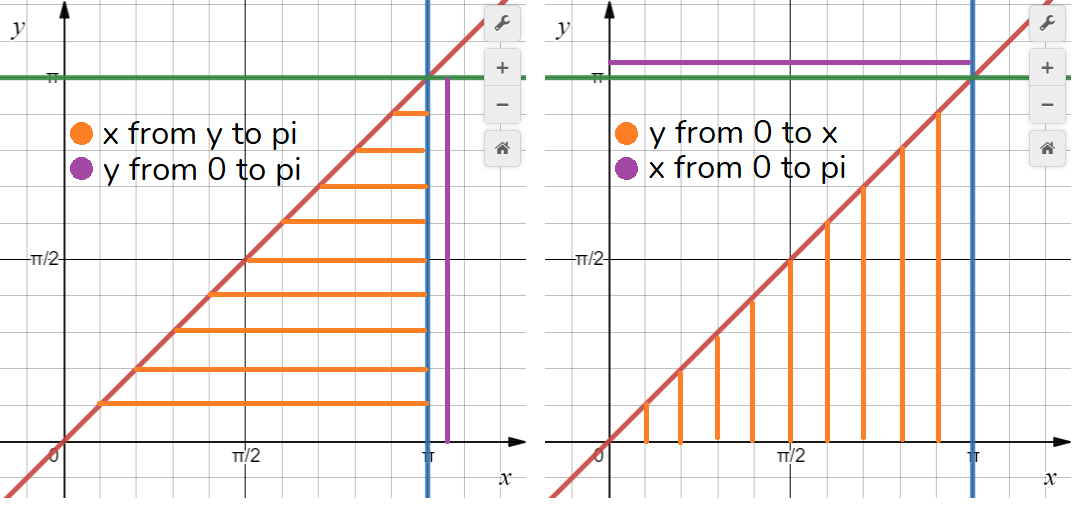
\includegraphics[width=\textwidth]{integration_area.png}
    \caption{On the left: original order of integration. On the right: inverted order of integration}
    \label{fig:integration_area}
  \end{figure}
